%!TEX root = /Users/markelikalderon/Documents/Git/formwithoutmatter/aristotle.tex
\chapter{Form Without Matter} % (fold)
\label{cha:form_without_matter}

\section{The Capacity to Assimilate} % (fold)
\label{sec:the_capacity_to_assimilate}

Color\index{color} is the power\index{power} to affect light\index{color!power to affect light}. This power grounds the derived power to mediately affect sense organs sensitive to such alterations. The eyes\index{eye} in seeing are filled with light. It is only by being illuminated that the transparent medium within\index{medium!internal} may be mediately acted upon by color. Extending the external light within triggers the reactive capacity for sight, the form and substance of the eye. In seeing the colors of external particulars\index{particular} arrayed in their environment the animal\index{animal} exercises their natural capacity to perceive and so realizes their nature as a perceiver. This is no alteration\index{alteration}. The perceiver both sees and has seen, perceptual activity being complete\index{complete} at every instant. In seeing the color of an external particular the perceiver, or perhaps their experience, becomes like the object of their visual experience actually is\index{assimilation!qualitative}. Perception is a mode of assimilation, though not as Empedocles\index{Empedocles} conceived of it. On the ingestion model\index{ingestion model}, assimilation is understood as a material mode of assimilation\index{assimilation!material}, the immediate object of sense, the emitted effluence\index{Empedocles!effluence}, being literally taken within the sense organ so that it may be in contact with the perceptive part of the soul. Perceptual activity, for Aristotle, may not be an instance of qualitative alteration\index{alteration}. Nevertheless, as in the case of alteration, the perceiver, or perhaps their experience, becomes like the way the perceived object\index{perception!object of} was prior to perception. The perceiver, or their experience, assimilates the sensible object in a manner necessarily distinct from the material assimilation of that object, since to be palpable is to be imperceptible. What is this non-material mode of assimilation? And how does it help resolve the Empedoclean puzzlement with which we began? These questions structure the present and final chapter. 

% section the_capacity_to_assimilate (end)

\section{The Wax Analogy} % (fold)
\label{sec:the_wax_analogy}

\index{wax analogy|(}
The assimilation of sensible form\index{assimilation!of sensible form}\index{form} without matter\index{matter}\index{assimilation!without matter} is explained in terms of an analogy with wax\index{wax} receiving the impression of a signet ring\index{signet ring}:
\begin{quote}
	Generally, about all perception, we can say that a sense is what has the power of receiving into itself the sensible forms of things without the matter, in the way in which a piece of wax takes on the impress of a signet-ring without the iron or gold; what produces the impression is a signet of bronze or gold, but not qua bronze or gold: in a similar way the sense is affected by what is coloured or flavoured or sounding not insofar as each is what it is, but insofar as it is of such and such a sort and according to its form. (Aristotle, \emph{De Anima} \textsc{ii} 12 424\( ^{a} \)18--23; Smith in \citealt[42--43]{Barnes:1984uq})\index{De Anima@\emph{De Anima}}
\end{quote}
Aristotle is explicit that the analogy is meant to hold of perception generally, as opposed to just vision or audition, say. A sense is what has the power\index{power} to assimilate the sensible form\index{assimilation!of sensible form} without the matter\index{assimilation!without matter} of a remote external particular\index{particular}. What does Aristotle mean by sense here? Does he mean the sense organ or the perceptual capacity the sense organ possesses, or at least endows the perceiver with? Given that Aristotle claims that a sense is what possesses this power, it is natural to understand him as having the sense organ in mind. So, for example, it is the eye\index{eye} that possesses the capacity to see\index{sight}, or at least endows their possessor with that capacity. In possessing or endowing the capacity to see, the eye potentially assimilates the color of remote external particulars.\index{assimilation!of sensible form}

Is the assimilation of sensible form\index{assimilation!of sensible form} a material change\index{change} that the eye undergoes in seeing, or is it a psychological change, the exercise of sight in seeing? Though Aristotle rejects the answer in the style of Gorgias\index{Emepdocles!answer in the style of Gorgias}, an echo of the ingestion model\index{ingestion model} remains in his optical anatomy. The eye in seeing is like a lantern\index{lantern}\index{Empedocles!lantern analogy}, not because it emits fire\index{fire!internal} from its interior, but because its interior is illuminated. The eye\index{eye}, being transparent\index{transparency}, admits the external light within, in the sense in which it can, light being a state\index{light!conceived as a state}, the state of illumination, and not a material body\index{body}. While a materially sufficient condition for the perceptual availability of a colored particular\index{particular}, it is merely a necessary condition for its perception. The wounded soldier's\index{wounded soldier} eyes are filled with light though he does not see since the passages leading\index{passages of the eye} within have been severed. While we have identified a material change that the eye undergoes in seeing\index{seeing}---its interior is illuminated---it is merely a necessary condition for sight's realization in seeing. The assimilation of sensible form by the eye is the exercise of the capacity that it endows its possessor with. So understood, it is the psychological change that the eye makes possible, the perceiver undergoing an episode of seeing, that the assimilation of sensible form is meant to characterize.

While denying that perception involves the assimilation of material effluences\index{assimilation!material}, Aristotle retains Empedocles'\index{Empedocles} conception of sensory awareness as a mode of assimilation, it is just that we assimilate form without matter. Indeed, this pattern of dialectical refinement\index{dialectical argument} continues in the very next line where Aristotle uses Plato's\index{Plato!wax analogy} metaphor of wax\index{wax} receiving an impression, not to characterize judgment as Plato\index{Plato} does in the \emph{Theaetetus} 194\( ^{c} \)--195\( ^{a} \),\index{Theaetetus@\emph{Theaetetus}} but to characterize the assimilation of sensible form\index{assimilation!of sensible form} in perception\index{perception}. The assimilation of sensible form is compared with the wax's reception of the impression\index{wax analogy} sealed by a signet ring\index{signet ring}. The wax\index{wax} receives the form imposed upon it by the signet ring\index{signet ring}, but it does not receive any of the matter that composes the ring, be it bronze\index{bronze} or gold\index{gold}, say. So, by analogy, when an animal\index{animal} perceives the white\index{white} of the sun\index{sun}, they assimilate the chromatic form of the sun but none of its matter. Moreover, just as it is the form of the ring\index{signet ring}, and not its gold\index{gold} or bronze\index{bronze}, that produces the sealed impression, its distinctive shape\index{shape}, it is the whiteness\index{white} of the sun\index{sun}, and not its matter\index{matter}, that produces the sensory impression, the perceptual experience of the white of the sun. We shall consider these points separately in the following subsections.
\index{wax analogy|)}

\subsection{Assimilation of Form} % (fold)
\label{sub:assimilation_of_form}

Aristotle's analogy is, significantly, of Platonic provenance. In the \emph{Theaetetus}\index{Theaetetus@\emph{Theaetetus}}, Plato\index{Plato} writes:
\begin{quotation}
	\textsc{socrates}: You will think better of it when you hear the rest. To judge truly is a fine thing and there is something discreditable in error.
	
	\textsc{theaetetus}: Of course.
	
	\textsc{socrates}: Well, they say the differences arise in this way. When a man has in his mind a good thick slab of wax\index{wax}, smooth\index{smooth} and knealed to the right consistency, and the impressions that come through the senses are stamped on these tables of the `heart'\index{heart}---Homer's\index{Homer} words hints at the mind's likeness to wax---then the imprints\index{impression} are clear and deep enough to last a long time. Such people are quick to learn and also have good memories,\index{memory} and besides they do not interchange the imprints of their perceptions\index{perception} but think truly. These imprints being distinct and well spaced are quickly assigned to their several stamps---the `real things' as they are called---and such men are said to be clever. Do you agree?
	
	\textsc{theaetetus}: Most emphatically.
	
	\textsc{socrates}: When a person has what the poet's wisdom commends as a `shaggy heart'\index{heart}, or when the block is muddy or made of impure wax\index{wax}, or oversoft\index{soft} or hard\index{hard}, the people with soft wax are quick to learn, but forgetful\index{forgetting}, those with hard wax, the reverse. Where it is shaggy\index{shaggy} or rough\index{rough}, a gritty\index{gritty} kind of stuff containing a lot of earth\index{earth} or dirt, the impressions\index{impression} obtained are indistinct; so are they too when the stuff is hard\index{hard}, for they have no depth. Impressions in soft\index{soft} wax\index{wax} also are indistinct, because they melt together and soon become blurred. And if besides this, they overlap through being crowded together into some wretched little narrow mind, they are still indistinct. All these types are likely to judge falsely. When they see or hear or think of something, they cannot quickly assign things to their several imprints. Because they are so slow and sort things into their wrong places, they constantly see and hear and think amiss, and say they are mistaken about things and stupid. (Plato, \emph{Theaetetus} 194\( ^{c} \)--195\( ^{a} \); Cornford in \citealt{Hamilton:1989fk})
\end{quotation}
Aristotle differs from Plato in:
\begin{enumerate}[(1)]
	\item what he uses the analogy for---to explain perception rather than judgment,\index{wax analogy}\index{Plato!wax analogy}
	\item the details of the analogy---in particular, the nature of the agent acting upon the wax, a signet ring\index{signet ring} as opposed to a stylus\index{stylus}, and
	\item how to understand the analogy---the way in which perceptions are meant to be like sealed impressions\index{impression} is different from the way in which judgments are like impressions made by styli.
\end{enumerate}
We shall consider these in turn. As will emerge, Aristotle's varying the agent acting upon the wax\index{wax}, his substitution of a signet ring\index{signet ring} for a stylus\index{stylus}, importantly bears on how he understands that analogy.

Whereas Plato deploys the wax analogy\index{Plato!wax analogy} to explain judgment\index{judgment}, Aristotle does so to explain perception. This difference is most likely intentional and pointed. First, Aristotle is a keen student of the \emph{Theaetetus}\index{Theaetetus@\emph{Theaetetus}} and discusses many of its arguments in a number of works. The variation is thus most likely intentional. But to what end? A second observation not only supports the first but sheds light on the significance of this variation. As we discussed in chapters~\ref{sec:definition} and \ref{sec:the_objects_of_perception}, and as \citet{Sorabji:1971fr,Sorabji:2003fk} emphasizes, Aristotle is extending the domain of perception as Plato conceives of it. Not only are the objects of perception\index{perception!objects of!primary} no longer confined to the primary objects---we perceive common\index{perception!objects of!common} and incidental\index{perception!objects of!incidental} sensibles as well---but Aristotle also maintains that we can discriminate among sensory objects and that this is the exercise of our perceptual capacities. Plato\index{Plato}, in contrast, maintained that what is ``common'' to the objects of sense---that they are each the same and different from the others---is determined by cognitive, not perceptual capacities. Aristotle underscores this extension of our perceptual capacities by his use of the Platonic analogy\index{Plato!wax analogy}. Aristotle emphasizes the fact that he is assigning to perception some of the functions that Plato assigns to judgment by using the analogy that Plato used to explain judgment to explain perception instead.

Another, perhaps less salient, difference between the Platonic and Aristotelian analogies concerns the nature of the agent acting upon the wax\index{wax}\index{wax analogy}\index{Plato!wax analogy}. Where\-as what makes an impression\index{impression} for Plato\index{Plato} is a stylus\index{stylus}, what makes an impression for Aristotle is a signet ring\index{signet ring}. Plato\index{Plato!wax analogy} has in mind a wax tablet\index{wax tablet}, used for writing\index{philosophy of mind and the technology of writing}, upon which characters are impressed with a stylus. Plato thus belongs to the Western tradition of using the then current writing technology as a model for the mind. Think of Locke's\index{Locke, John} blank slate\index{blank slate}, or the functionalist\index{functionalism} slogan that the mind is the software of the brain\index{mind as the software of the brain}, itself coinciding with the emergence of text-editing\index{text-editing} and word-processing\index{word-processing}. That thought has the grammatical\index{grammar} structure of written language, developed in different ways by Ockham\index{Ockham, William} and Fodor\index{Fodor, Jerry}, is a close variation. As is Lacan's\index{Lacan, Jacques} claim that the unconscious\index{unconscious} is structured like a language, at least if we regard analysis\index{analysis} as a discursive technology. Perhaps Nietzsche\index{Nietzsche, Friedrich} was right that our writing tools act upon our thoughts. They at least have a tendency to influence our philosophy of mind. Aristotle varies this aspect of the Platonic analogy\index{Plato!wax analogy}. It is not a stylus\index{stylus} on a wax tablet\index{wax tablet} that creates the impression\index{impression}, it is a signet ring\index{signet ring}. Why the substitution? I believe the variation is intentional. Both a stylus and a signet ring are involved in the production of writing. The difference concerns their distinctive discursive roles\index{discursive roles}. The significance of this discursive difference will emerge in sequel. 

Not only does Aristotle deploy the Platonic analogy\index{Plato!wax analogy}, varied in this way, to explain his conception of perception, but, importantly, he also transforms how the analogy is understood. Plato's explanation of the reliability of memory\index{memory} and judgment\index{judgment} crucially relies on causal features of the situation. An objects' impression\index{impression} is the effect it has on the mind's wax. Importantly, however, Aristotle has in mind a non-causal sense of impression. As we shall see, the distinctive discursive role of signet rings will bear on the sense in which a ring's seal is an impression.

To get a sense of this contrast, first consider how Hume\index{Hume, David} himself appropriates the Platonic analogy\index{Plato!wax analogy}:
\begin{quote}
	All the perceptions of the human mind resolve themselves into two distinct kinds, which I shall call \textsc{impressions}\index{impression} and \textsc{ideas}\index{idea}. The difference betwixt these consists in the degree of force or liveliness, with which they strike upon the mind, and make their way into thought and consciousness. (\citealt{Hume:1739kx}, \emph{Treatise} \textsc{i} 1 1 1)\index{A Treatise of Human Nature@\emph{A Treatise of Human Nature}}
\end{quote}
Hume begs his reader's indulgence in taking liberty with the use of the terms ``impression'' and ``idea'' (\citealt{Hume:1739kx}, \emph{Treatise} \textsc{i} 1 1 n2) though he claims that it is at least a virtue of his regimentation that it ``restore[s] the word, \emph{idea}, to its original sense, from which Mr. \emph{Locke}\index{Locke, John} had perverted it, in making it stand for all our perceptions.'' Hume\index{Hume, David} is presumably taking liberty with his use of the term ``perception'', as well. Locke perverts the use of ``idea'' by making it stand for all perceptions. But perception, here, is not a sensory experience, nor is it confined to the objects of sensory experience. By ``perception'' Hume means whatever is or could be set before the mind (in, admittedly, a post-Cartesian conception of mind unavailable to the ancients). The perceptions present to the human mind are either impressions or ideas, depending upon the force or liveliness with which they strike the mind. Impressions\index{impression} are the objects that are presented with ``the most force and violence'' (\citealt{Hume:1739kx}, \emph{Treatise} \textsc{i} 1 1 1).  Concerning impressions, Hume further explains:
\begin{quote}
	By the term \emph{impression} I wou'd not be understood to express the manner, in which our lively perceptions are produc'd in the soul, but merely the perceptions themselves; for which there is no particular name either in \emph{English} or any other language, that I know of. (\citealt{Hume:1739kx}, \emph{Treatise}, \textsc{i} 1 1 n2)
\end{quote}
Consistent with this qualification, Hume is, nevertheless, operating with a causal notion of impression. The lively perceptions presented before the mind in viewing the streets of Edinburgh\index{Edinburgh} are themselves the effects of external causes. Inquiring after the manner in which such lively perceptions are produced in the soul\index{soul} does not, however, fall within the purview of Hume's new science of human nature\index{Hume, David!new science of human nature}. It belongs, rather, to a particular branch of natural philosophy, speculative anatomy\index{Hume, David!speculative anatomy}. The qualification is not the denial that impressions are effects. It rather signals Hume's intention to confine himself to what might be described in a later terminology as the phenomenology\index{phenomenology}, the intentional objects of consciousness, in particular, to the few regular principles that govern the persistent change among the perceptions present before the mind.

Like Aristotle, Hume\index{Hume, David} is departing from Plato in using the analogy of impressions on wax to describe perceptual experience (and more besides, passions are impressions as well). But Hume retains a key feature of Plato's original use of the analogy\index{Plato!wax analogy}. Hume is still thinking of sensory impressions\index{impression} as the effects produced in the perceiver by external objects acting upon them. Is there an intelligible alternative? How else might talk of impressions be understood? 

Consider the closely related metaphor of shaping.\index{shaping} There is clearly a causal sense of shaping\index{shaping!causal}. When the stylus\index{stylus} shapes the wax tablet\index{wax tablet} it causes the wax\index{wax} to be modified in a certain way. The wax takes on the shape imposed upon it by the stylus. Similarly, Nazi bombing\index{Nazi bombing} shaped the London\index{London} skyline. It caused that skyline to be configured in a certain way, the way imposed upon it by the bombing. Importantly, however, there is another sense of shaping, not a causal sense, but a constitutive sense\index{shapting!constitutive}. Whereas Nazi bombing\index{Nazi bombing} shaped the London\index{London} skyline merely in a causal sense, St Paul's\index{St Paul's} constitutively shapes\index{shaping!constitutive} that skyline by being a contour of it. This is dramatically demonstrated in Herbert Mason's\index{Mason!Herbert} iconic photograph of St Paul's\index{St Paul's} on 29 December 1940. St Paul's defiantly shapes the London skyline by being a part of it, despite the devastating impact of Nazi bombing\index{Nazi bombing}.

%  (see figure~\ref{fig:stpauls})
% \begin{figure}[htbp]
% 	\centering
% 		
\includegraphics[scale=0.6]{graphics/stpauls.jpg}
% 	\caption{St Paul's 29 December 1940}
% 	\label{fig:stpauls}
% \end{figure}

Humean\index{Hume, David} sensory impressions\index{impression} are shaped by the environment merely in a causal sense. This is central to Hume's use of the Platonic analogy. Just as a stylus\index{stylus} impinging upon the wax\index{wax} causes an impression, the environment impinging upon a perceiver with the appropriate sensory capacities causes a sensory impression. How exactly such sensory impressions are produced is a matter for the speculative a\-na\-to\-mist\index{Hume, David!speculative anatomy}. Hume's new science of human nature\index{Hume, David!new science of human nature} confines itself to sensory impressions and the regularities that can be discerned in the flux\index{flux} of sensory experience. But sensory impressions, episodes in the sensory flux, remain effects, nonetheless. But perhaps perceptual sensitivity is more than the environment impinging upon the state of a conscious subject. Perhaps there is more to perception than objects eliciting a conscious modification of the perceiving subject. Perhaps the environment can shape sensory consciousness in a constitutive, rather than merely a causal, sense.

Before exploring this idea further, let us consider another important, and importantly related, aspect of Aristotle's use of the Platonic analogy\index{Plato!wax analogy}\index{wax analogy}. Earlier we observed that Aristotle varies the Platonic analogy by substituting a signet ring\index{signet ring} for Plato's stylus\index{stylus}. What is the significance of this variation? Both are involved in the production of writing. The difference lies in their distinctive discursive roles. Caston\index{Caston, Victor} observes that the impression produced by a signet ring\index{signet ring} is linked to that particular ring and, hence, metonymically at least, to the legitimate possessor of that ring:\index{discursive roles}
\begin{quote}
	A signet\index{signet ring} produces a sealing, an impression\index{impression} that establishes the identity of its owner and consequently his authority\index{authority}, rights, and prerogatives. When a sealing is placed on a document, especially for legal or official use, it authorizes the claims, obligations, promises, or orders made therein. A sealing thus differs from other impressions in that it \emph{purports to originate from a particular signet}. \citep[302]{Caston:2005cr}
\end{quote}
The impression of a signet ring\index{signet ring} thus plays a similar role to signatures\index{signature}. Just as a signature is linked to the particular person whose signature it is, the impression sealed upon the wax by a signet ring is linked to the legitimate possessor of that ring. Moreover, signatures, like sealed impressions, carry a certain authority\index{authority}, the authority endowed by their legitimate possessors. Of course, signatures can be forged, as can signet rings, which can also be stolen, but these practices gain there point precisely by the link between a signature and sealed impression, on the one hand, and their legitimate possessors, on the other. Signet rings and styli thus have distinctive discursive roles\index{discursive roles}. The impression made by a stylus is not linked to its legitimate possessor---one scribe may borrow another's stylus---the way an impression sealed by a signet ring\index{signet ring} is.

Taking this feature of the analogy\index{wax analogy} seriously has an important consequence for how sensory impressions are individuated. Just as a forged signature is not my signature\index{signature}, an impression\index{impression} sealed by a forged ring, or by a stolen ring, is not the seal of the ring's legitimate possessor. Impressions are individuated by their legitimate sources. If this feature of the analogy carries over, then perceptions, conceived on the model of sealed impressions\index{impression}, are individuated by their objects which are their source. A perception of Castor\index{Castor} and a perception of Pollux\index{Pollux} are different perceptions, no matter how closely the twins may resemble one another. Just as a forged seal is not my seal, a perception of Castor is not a perception of Pollux. A forged seal may be a perfect duplicate of a genuine seal but it is not the seal of the ring's legitimate possessor. Castor may be a perfect duplicate of Pollux, but my visual impression of Castor is not an impression of Pollux. 

Notice that a causal understanding of sensory impressions\index{impression}\index{shaping! causal}, as merely the effects of causal shaping, does not have this consequence. If, as Hume maintained, cause and effect are contingently connected, the same effect, the same impression, could have been produced by a different cause. Sensory impressions, understood as the effects of causal shaping, are not individuated by their causes. If sensory impressions are individuated by their objects which are their sources, they cannot be understood as merely the effects of causal shaping. How else might they be understood?

If sensory impressions are individuated by their objects, perhaps these objects shape sensory consciousness not causally, or at least not merely. Perhaps in being individuated by their objects, these objects constitutively shape\index{shaping!constitutive} our sensory impressions\index{impression} of them (for contemporary discussion of this suggestion see \citealt{McDowell:1998vn,Martin:2004fj,Fish:2009fk,Kalderon:2011fk}). Looking up, you see the brilliance of the late morning sun\index{sun} burning white\index{white}. The whiteness of the sun is a constituent of your experience. Sensory experience is an encounter with, at least, its primary objects\index{perception!object of!primary}. In sensory consciousness, we simply confront the primary object of the given modality. We cannot be confronted truly or falsely, correctly or incorrectly (discussed in chapter~\ref{sec:the_objects_of_perception}). We simply encounter what is presented to us in sensory consciousness. The whiteness\index{white} of the sun\index{sun} is a constituent of your experience insofar as that experience involves the presentation of that whiteness in the visual awareness afforded you by your experience of the sun. And since your experience is constitutively linked to the whiteness of the sun, the sun's whiteness, whose brilliance can inspire both glory and terror, shapes the contours of your visual consciousness by being present in that consciousness.\index{shaping!constitutive} The whiteness\index{white} of the sun\index{sun} shapes the contours of your visual experience in the way that St Paul's\index{St Paul's} defiantly shapes the London\index{London} skyline, the Shard\index{the Shard} notwithstanding, simply by being present. The whiteness\index{white} of the sun\index{sun} is present in the awareness that sight\index{sight} affords you of the scene. That experience has a certain character. The character of that experience depends upon and derives from the character of the presented whiteness\index{white}. Your experience, in this sense, becomes like the way the sun\index{sun} actually is, brilliant white. Just as what the London\index{London} skyline is like depends, in part, upon what St Paul's\index{St Paul's} is like, since the London skyline involves the presence of St Paul's as a part, what your experience of the sun is like depends, in part, upon what the sun's whiteness is like, since your experience involves the presentation in sight of that whiteness.

We are now in a position to state, in a preliminary fashion, what the doctrine of the assimilation of sensible form\index{assimilation!of sensible form} amounts to. In seeing the white\index{white} of the sun\index{sun}, the perceiver assimilates the chromatic form of that heavenly body, where the assimilation of chromatic form is the white of the sun constitutively shaping\index{shaping!constitutive} the perceiver's experience of it. If the white of the sun constitutively shapes the perceiver's experience of it, then the sun must be actually white. Not only does perception thus existentially depend\index{existential dependence}, in this way, upon its object, but perception ontologically depends\index{ontological dependence} upon its object as well (on ontological dependence see \citealt{Fine:1995ls}, on ontological dependence and Aristotle see \citealt{Peramatzis:2011aa}). What it is for a perceptual experience to be the perceptual experience it is depends upon what it is for its object to be the kind of thing it is. Though Aristotle's focus throughout is on the primary sensibles\index{perception!object of!primary}, it is plausible that this thesis holds for the class of objects that are perceptible in themselves\index{perceptible!in themselves} and thus for common sensibles\index{perception!object of!common} as well, if not for incidental sensibles\index{perception!object of!incidental}. The doctrine of the assimilation of sensible form\index{assimilation!of sensible form} is arguably a consequence of this more general claim and the qualitative character of objects that are perceptible in themselves. The primary objects of sight are perceptible in themselves. The primary objects of sight are the colors\index{color!primary object of sight} and the luminous\index{the luminous}---visible qualities that inhere in particulars\index{particular}. And what it is to be the white\index{white} of the sun\index{sun} is a matter of the qualitative character determined by the sun's power to produce light\index{light}, to make what was potentially transparent actually transparent\index{transparency}. So the perception\index{perception} of the white of the sun ontologically depends\index{ontological dependence} upon something whose being consists in its qualitative character.  As a consequence, the character of the perceptual experience---in Nagel's \citeyearpar{Nagel:1979fk}\index{Nagel, Thomas} terminology, what it is like for the perceiver to undergo that experience (for doubts about the Nagelian idiom see \citealt{Snowdon:2010ap}\index{Snowdon, Paul})---depends upon and derives from what the sun\index{sun} is actually like, burning white\index{white}. 

The doctrine of the assimilation of sensible form\index{assimilation!of sensible form} is an elaboration of the conception of sensory presentation\index{presentation} at work in the viewpoint conception of perceptual experience\index{perception!viewpoint conception} that underwrote Aristotle's rejection of the Empedoclean principle\index{Empedocles!the Empedoclean principle} (for contemporary defenses of the viewpoint conception see \citealt{Martin:1998nx}\index{Martin. M.G.F.} and \citealt{Kalderon:2011fk}). Aristotle claimed that vision could not be explained in terms of contact with the visible since a colored particular's\index{particular} contact with the receptive part of the eye\index{eye} blinds the perceiver to the particular and its color. In order to see a colored particular, the perceiver must have a point of view on it\index{perception!point of view}, and this requires that the perceived object be at a distance from the organ of sight (chapter~\ref{sec:against_the_empedoclean_principle})\index{perception at a distance}. On the viewpoint conception of perceptual experience\index{perception!viewpoint conception}, perception just is the presentation\index{presentation} of its object to the perceiver's point of view. So what it is like for the perceiver to undergo such an experience is determined, at least in part, by what the presented object is like. And that just is the relevant notion of qualitative assimilation\index{assimilation!qualitative} at work in perception.

The present interpretation of the doctrine of assimilation of sensible form\index{assimilation!of sensible form} was said to be preliminary since it remains subject to both qualification and elaboration. Let me mention four points that require further elaboration: (1) In seeing the white\index{white} of the sun\index{sun}, the perceiver's perceptual experience becomes like the sun actually is, brilliant white, but it does not become exactly like the sun's brilliance. How are we to understand this? (2) Part of this difference concerns the contribution of the perceiver's point of view\index{perspective} to what it is like for the object of perception to be presented to that point of view. How is the contribution of the perceiver's point of view to be understood within the Aristotelian framework? (3) More fundamentally, we have yet to examine Aristotle's qualification, essential to resolving the generalized form of Empedoclean puzzlement\index{Empedoclean puzzlement!general form}, that the perceiver assimilates the chromatic form\index{form} of the distant sun without its matter\index{matter}.\index{assimilation!without matter} (4) Aristotle claims that plants\index{plant} are insensate to temperature\index{temperature} because they lack a mean\index{mean}. What, if anything, does this tell us about the general nature of sensory presentation\index{presentation}? The first two points will be discussed in the remainder of this section. The third and fourth points will be discussed in the following two sections, \ref{sub:without_matter} and \ref{sub:sensory_presentation_as_a_mean}, respectively.

What the London\index{London} skyline is like depends, in part, upon what St Paul's\index{St Paul's} is like since the London skyline involves the presence of St Paul's as a part. But the way in which the brilliant white\index{white} of the sun\index{sun} is present in your experience is not the way St Paul's is present in the London skyline. The brilliant white of the sun is not a part of your experience, though it may be a constituent. The white of the sun and St Paul's are present in different ways and this makes for a corresponding difference in the sense of likeness that their presence grounds. Thus the London\index{London} skyline is actually like St Paul's\index{St Paul's} in that it shares a common contour, say. But neither the perceiver nor their perceptual experience becomes actually white\index{white} in assimilating the chromatic form of the sun\index{assimilation!qualitative}. The perceiver, or the perceptual experience, may be like the way the sun actually is, brilliant white, but this does not require that they or their experience be actually white. Echoing \citet{Austin:1962lr}\index{Austin, J.L.} we might say, just because the perceiver, or their perceptual experience, becomes like the perceived object actually is does not mean that they become exactly like the perceived object. In seeing the white\index{white} of the sun\index{white}, the character of your perceptual experience depends upon and derives from the character of color presented to your point of view. But this requires neither that the perceiver nor their perceptual experience actually take on the color\index{color} of the perceived particular\index{particular}.

Consider, again, assimilation\index{assimilation!qualitative} as it figures, not in perception, but in the production of artifacts\index{artifact}. In the perceptual case, the perceiver assimilates the form of the perceived object. In the production of artifacts, the direction of assimilation is reversed. It is not a person assimilating the form of an external object, but an external object assimilating a form that is in some sense in the person. The iron in being forged into a sword takes on or assimilates the form contained in the soul\index{soul} of the person possessing the art\index{art}.  But there is no actual sword\index{sword} in the smith’s\index{swordsmith} soul. So, in seeing the brilliant white of the sun\index{sun}, the perceiver may become like the sun actually is, but there need not be within them anything brilliant white\index{white}.

Moreover, qualitative assimilation\index{assimilation!qualitative} in the case of vision\index{sight} is relative to a point of view\index{perspective}. But the qualitative alteration of natural bodies\index{body} need not be relative in this way, and Aristotle's paradigmatic examples of alterations display no such relativity. That vision requires a point of view was the basis of Aristotle's case against the Empedoclean principle\index{Empedocles!the Empedoclean principle}. One can only see from a given point of view\index{perspective}, but this, in turn, requires that the object seen be distant from the perceiver. Moreover the directionality of the visible, at work in occlusion\index{occlusion}, shadow\index{shadow}, and reflection\index{reflection}, is determined, in part, by a point of view that a perceiver could occupy. The same sensory object may be presented to different point of views\index{perspective}. In being presented to different points of view, the corresponding experiences would themselves differ in character. Thus the color a mountain\index{mountain} presented through an imperfectly transparent sky may be seen from near and from far. Seen near the mountain looks one way, seen far it looks another. Do these appearances conflict? Aristotle expresses surprise that the question could even arise whether ``colors are of such a nature such as they appear to people at a distance\index{distance}, or as they appear to those close at hand'' (\emph{Metaphysica} \( \Gamma \) 5 1010\( ^{b} \)4--5; Ross in \citealt[55]{Barnes:1984kx})\index{Metaphysica@\emph{Metaphysica}}. The same color\index{color} presented to different points of view will look different, but this difference in look or appearance is not explained by a difference in what is presented. The different look of the mountain's\index{mountain} color seen near and far is its color being presented to different points of view. Crimson\index{crimson} just is what white radiant light sources look like when seen through smoke-filled media, a look they do not have when seen, unobscured, from other points of view.

In chapter~\ref{sec:the_definition_of_color} we saw how this perspectival relativity\index{perspective} can be explained consistent with color materially altering illuminated media\index{medium}. Suppose a Heraclitean metaphysics of fire\index{Heraclitus!fire} were right to the extent that for fire\index{fire}, at least, to be is to burn. Then since the presence of the fiery substance\index{fiery substance} makes a potentially transparent\index{transparency} medium\index{medium} actually transparent, this is wholly due to the activity of the fiery substance\index{fiery substance}. The being of the fiery substance consists in its burning, understood as the general activity of fire, and the specific way that it burns. A color's effect on the illuminated medium consists in the growth or diminution of the activity of the fiery substance. Activities, however, have a direction of influence.\index{fiery substance!direction of influence} Since the illuminating activity of the fiery substance\index{fiery substance} renders visible the colored\index{color} particulars\index{particular} arrayed within the transparent\index{transparency} medium\index{medium}, the directionality of the visible\index{the visible!directionality of} is ultimately explained by the direction of influence of the fiery substance\index{fiery substance!direction of influence}. Actual transparency\index{transparency}, though a relatively stable state\index{state} of the medium\index{medium}, may nevertheless have a direction it inherits from its determinant, the illuminating activity of the fiery substance.

Consider how the direction of influence of the fiery substance\index{fiery substance!direction of influence} can help explain the variation of color\index{color} appearance with distance. The mountain's\index{mountain} color alters the imperfectly transparent\index{transparency} medium\index{medium} by altering the extent and the activity of the fiery substance\index{fiery substance}. The medium, in being imperfectly transparent, limits color's power, however. In an imperfectly transparent medium, color has a limited sphere of influence\index{color!limited sphere of influence}. Within that sphere, when the perceiver is near the colored particular\index{particular}, color alters the imperfectly transparent in such a way that it is visible within the medium. But outside that sphere, when the perceiver is too distant from the colored particular, the color of the particular does not alter the imperfectly transparent medium such that it is visible in that medium, at least not from the perceiver's point of view. Moreover, not only is color's power limited but within its limited sphere it is variable as well. Here, the directed influence of the fiery substance\index{fiery substance}, its extent and degree of activity having been acted upon by the color, is impeded by the composition of the imperfectly transparent medium\index{medium}. Just as, in the case of the sun seen through a cloud of smoke, the influence of the sun's\index{sun} radiance is impeded by black\index{black} particulate matter\index{matter} suspended in the air\index{air}. And just as in the case of the sun\index{sun}, the impediment to incorporeal activity\index{fiery substance!incorporeal activity}, a rarefied form of burning, posed by the imperfectly transparent medium affects the appearance of colors seen through it. Red\index{red} is what radiant white\index{white} things look like when seen through smoke-filled\index{smoke} media, and blue\index{blue} is what mountains\index{mountain} look like seen at a distance through an imperfectly transparent sky.

In perceiving the color\index{color} of a remote external particular\index{particular}, the perceiver assimilates that particular's chromatic form. While many commentators understand the assimilation of chromatic form as a kind of causal shaping\index{shaping!causal}, the proposal is that we instead understand the assimilation of chromatic form as the presented color's constitutively shaping\index{shaping!constitutive} visual experience. In being present in the awareness afforded by visual experience, the color constitutively shapes that experience. The character of that experience depends upon and derives from the character of the color presented to the perceiver's point of view\index{perspective}. In this sense does color experience become like the presented color. And in this sense is the perceiver, or at least their perceptual experience, potentially like the colored particular actually is prior to perception (in the sense discussed in chapter~\ref{sub:external}).

% subsection assimilation_of_form (end)

\subsection{Without Matter} % (fold)
\label{sub:without_matter}

\index{assimilation!without matter|(}
In perception\index{perception}, not only do we assimilate the sensible form\index{assimilation!of sensible form} of the object of perception, but we do so without assimilating any of its matter\index{matter}. This is a direct consequence of Aristotle's case against the Empedoclean principle\index{Emedocles!the Empedoclean principle}, to be perceptible is to be palpable to sense (discussed in chapter~\ref{sec:against_the_empedoclean_principle}). If contact with the sense organ precludes sensation, then the assimilation of anything material by the organ of sensation would be incompatible with the exercise of our perceptual capacities. Concerning this, Aristotle uses the analogy to make two remarks:
\begin{enumerate}[(1)]
	\item that the wax\index{wax} takes on the impression\index{impression} of the signet ring\index{signet ring} without the bronze\index{bronze} or gold\index{gold}, and
	\item that the bronze\index{bronze} or gold\index{gold} signet ring\index{signet ring} produces the impression\index{impression}, but not \emph{qua} bronze or gold.
\end{enumerate}

First, in sealing, the signet ring\index{signet ring} makes an impression\index{impression} upon the wax\index{wax}\index{wax analogy}. The wax takes on the seal\index{seal}, the form\index{form} imposed upon it by the signet ring\index{signet ring}. However, the wax does not take on any of the matter\index{matter} that composes the ring.  The contribution of the ring to the sealed impression is exhausted by the form it imposes. The ring makes no further material contribution to the sealed impression. It leaves no deposits of gold\index{gold}. This feature of the analogy is the summation of Aristotle's case against the Empedoclean principle\index{Empedocles!the Empedoclean principle}. Perception may be a mode of assimilation, but it is not the assimilation\index{assimilation!material} of anything material. In the case of qualitative alteration\index{alteration}, as Aristotle understands it, nothing material is assimilated. What is assimilated is not a body, but a quality or state.\index{assimilation!qualitative} And as I have observed in chapter~\ref{sec:transparency_in_de_anima}, whereas bodies\index{body} have locations\index{location}, qualities\index{quality} and states\index{state} do not. Perceptual activity may not be an instance of qualitative alteration,\index{alteration} nevertheless, as in the case of alteration, the perceiver, or perhaps their experience, becomes like the way the perceived object actually is. The perceiver, or their experience, assimilates the sensible form\index{assimilation!of sensible form} of the perceived particular in a manner necessarily distinct from the material assimilation of that particular, since to be palpable is to be imperceptible.

Second, the bronze\index{bronze} or gold\index{gold} signet ring\index{signet ring} produces the impression\index{impression} but not \emph{qua} bronze or gold. Aristotle is characteristically brief in his statement of this claim, which requires some explanation. After all, it is not as if being made of bronze or gold has nothing to do with the power\index{power} to produce impressions\index{impressions} upon wax\index{wax}. As Plato's\index{Plato} elaboration of the wax analogy makes clear, to impress a form upon the wax requires that the agent of this change be sufficiently hard\index{hard} and rigid\index{rigid}. Styli\index{stylus} and signet rings\index{signet ring} could not be composed of water\index{water}, say, because water lacks fixed boundaries\index{unbounded} and so would lack the requisite rigidity. Let the capacity to impose a sealed impression\index{impression} upon wax be the form of a signet ring. There may be material constraints on sustaining that form\index{form}. Perhaps only matter with certain elemental\index{elements} compositions could be signet rings. Consistent with this, Aristotle is making the further claim that when the bronze\index{bronze} or gold\index{gold} signet ring\index{signet ring} acts upon the wax\index{wax} to produce the sealed impression\index{impression}, the ring is acting but not \emph{qua} bronze or gold. Aristotle's idea seems to be this. Being made of bronze\index{bronze} or gold\index{gold} may contribute to the requisite hardness and rigidity of a signet ring\index{signet ring}. But when that ring seals an impression\index{impression} upon the wax, the wax takes on the form it does, less because of the golden composition of the ring, say, than because of its shape. To sustain that shape sufficient to impress a recognizable form upon wax may place material constraints on what the ring could be made of. A ring with the same shape could be made of iron or bronze, say, but not of water\index{water}. But what explains the form that the wax\index{wax} takes on is primarily the shape of the ring that imposes that form.\index{wax analogy}

How would this feature of the analogy carry over to the case of perception?

Vision is an encounter with the visible\index{the visible}. Looking up you are momentarily dazzled by the brilliance of the late morning sun\index{sun}. In seeing the sun, you encounter the sun's brilliant whiteness\index{white}. The sun's whiteness is the primary object of your visual experience\index{perception!object of!primary}. And it is for the sake of presenting the primary objects of vision---the visible, colors\index{color} in light\index{light} and the luminous\index{the luminous} in dark\index{dark}---that you possess eyes\index{eye} to see with. The sun's\index{sun} brilliant whiteness\index{white} is the power\index{power} of the sun\index{sun} to act on what is actually transparent. Although, in the case of the sun, given the strength of its illumination, the sun is also the cause of daylight. The sun does not merely have the power to alter what is actually transparent\index{transparent}, but it also has the power to make what is potentially transparent actually transparent. The whiteness\index{white} of the sun\index{sun} is the sun's power\index{power} to affect light in a certain way, to both produce it and endow it with a certain character. In possessing the power to affect light in this way, the sun also possesses the power to mediately affect organs of sensation sensitive to such alterations\index{alteration} in illuminated media. The whiteness\index{white} of the late morning sun, in all its brilliance, is the cause of its presentation\index{presentation} in your visual experience. What explains your taking in the sun's color\index{color} is the sun's\index{sun} brilliant whiteness\index{white} being open to your view. Just as the signet ring\index{signet ring} must have the shape\index{shape} it has prior to imposing its form\index{form} upon the wax\index{wax}, a particular must have the color that it has prior to its chromatic form being assimilated in visual perception. And just as it is the shape of the signet ring\index{signet ring}, and not its matter\index{matter}, that primarily explains the form that it imposes upon the wax\index{wax}, it is the color\index{color} of the particular\index{particular} and not its matter\index{matter} that primarily explains the chromatic form assimilated\index{assimilation!of sensible form}, the color's presentation\index{presentation} in visual consciousness. (For contemporary defense of the claim that colors are explanatorily indispensable in the production of color experience see \citealt{Campbell:1997dq,Broackes:1997pa,Yablo:1995fk}; for related discussion in Aristotle scholarship see \citealt{Broadie:1993fk,Broackes:1999uq})\index{wax analogy}

Previously, we distinguished causal and constitutive senses of shaping\index{shaping!causal}\index{shaping!constitutive}. Something may causally shape a thing by causing it to have a certain shape\index{shape}. But, importantly, something may constitutively shape a thing, by being a part, or contour, of that thing's shape. I suggested that we might understand the doctrine of the assimilation of sensible form\index{assimilation!of sensible form} in terms of the primary objects\index{perception!objects of!primary} constitutively shaping\index{shaping!constitutive} sensory consciousness. In experiencing the sun's\index{sun} brilliant whiteness\index{white}, the sun's chromatic form constitutively shapes\index{shape!constitutive} your visual experience by being present in the awareness that it affords. How does this square with Aristotle's insistence that the assimilation of sensible\index{assimilation!of sensible form} form is the product of the sensible form assimilated?\index{wax analogy}

In claiming that the sun's\index{sun} brilliant whiteness\index{white} constitutively shapes\index{shaping!constitutive} your visual experience, the contrast is with the sun's\index{sun} whiteness\index{white} merely causally shaping\index{shaping!causal} that experience. The sun's\index{sun} brilliant whiteness\index{white} consist in its power\index{power} to affect light\index{light} in a certain way, to both produce it and endow it with a certain character. The sun possesses this power prior to being perceived. Indeed it must possess this power prior to perception since it is the cause of that perception, and so must be actually like the perceiver's experience potentially is. The sun's brilliant whiteness is presented\index{presentation} in the awareness that your visual experience affords you of the sun. The sun's whiteness shapes the contours of your visual experience by being present in the awareness that it affords. Consistent with its constitutively shaping visual consciousness, the sun's\index{sun} brilliant whiteness\index{white} brings about its presentation in your consciousness, by altering your eye's\index{eye} interior illumination and so triggering your reactive capacity for sight. The first actuality of color is the cause, in appropriate circumstances, of the second actuality of color, its presentation in visual consciousness. So the primary object of sight\index{sight}, color, causes a suitably placed, awake, and attentive perceiver to stand in a certain relation to it, that of visual awareness. And in standing in that relation, in being presented in visual awareness, the color constitutively shapes the perceiver's visual experience. The object of perception is a cause that brings it about that a perceiver is perceptually related to it, like a wind causing a fire to burn in its direction.

Colors may be causes, but that does not make the shaping of visual experience by color merely causal\index{shaping!constitutive}\index{shaping!causal}. The sun's\index{sun} whiteness\index{white} may elicit a perception of it in suitably placed, awake, and attentive viewers, but what that perceptual experience is like depends upon and derives from what the sun is actually like prior to perception, namely, brilliant white. If color shaped visual experience in a merely casual sense this latter conjunct would not be true. Consider Descartes'\index{Descartes, Ren\'{e}} striking and paradoxical comparison, in the \emph{La Dioptrique}\index{La Dioptrique@\emph{La Dioptrique}}, of color vision with a blind person's use of a stick\index{blind person's stick} in navigation. Part of the point of the comparison is that there need be nothing in the objects which resembles the ideas or sensations that we have of them (\emph{La Dioptrique}, First Discourse)\index{Descartes, Ren\'{e}!resemblance thesis}. Descartes is here supposing that colors are the ways that bodies receive light and reflect it against our eyes (\emph{La Dioptrique}\index{La Dioptrique@\emph{La Dioptrique}}, First Discourse).\index{Descartes, Ren\'{e}!color} Nevertheless, he maintains that our sensations of color do not resemble the colors that elicits them. Colors, according to Descartes, shape sensory consciousness merely causally since there is nothing in the colored particular that resembles our visual impression\index{impression} of it. Descartes'\index{Descartes, Ren\'{e}} claim, here, is representative of a dominant theme in early modern thinking about sensory experience that coincides with an emerging consensus that colors are, in some suitable sense, secondary qualities\index{secondary qualities}.

% (see figure~\ref{fig:blind})
% \begin{figure}[htbp]
% 	\centering
% 		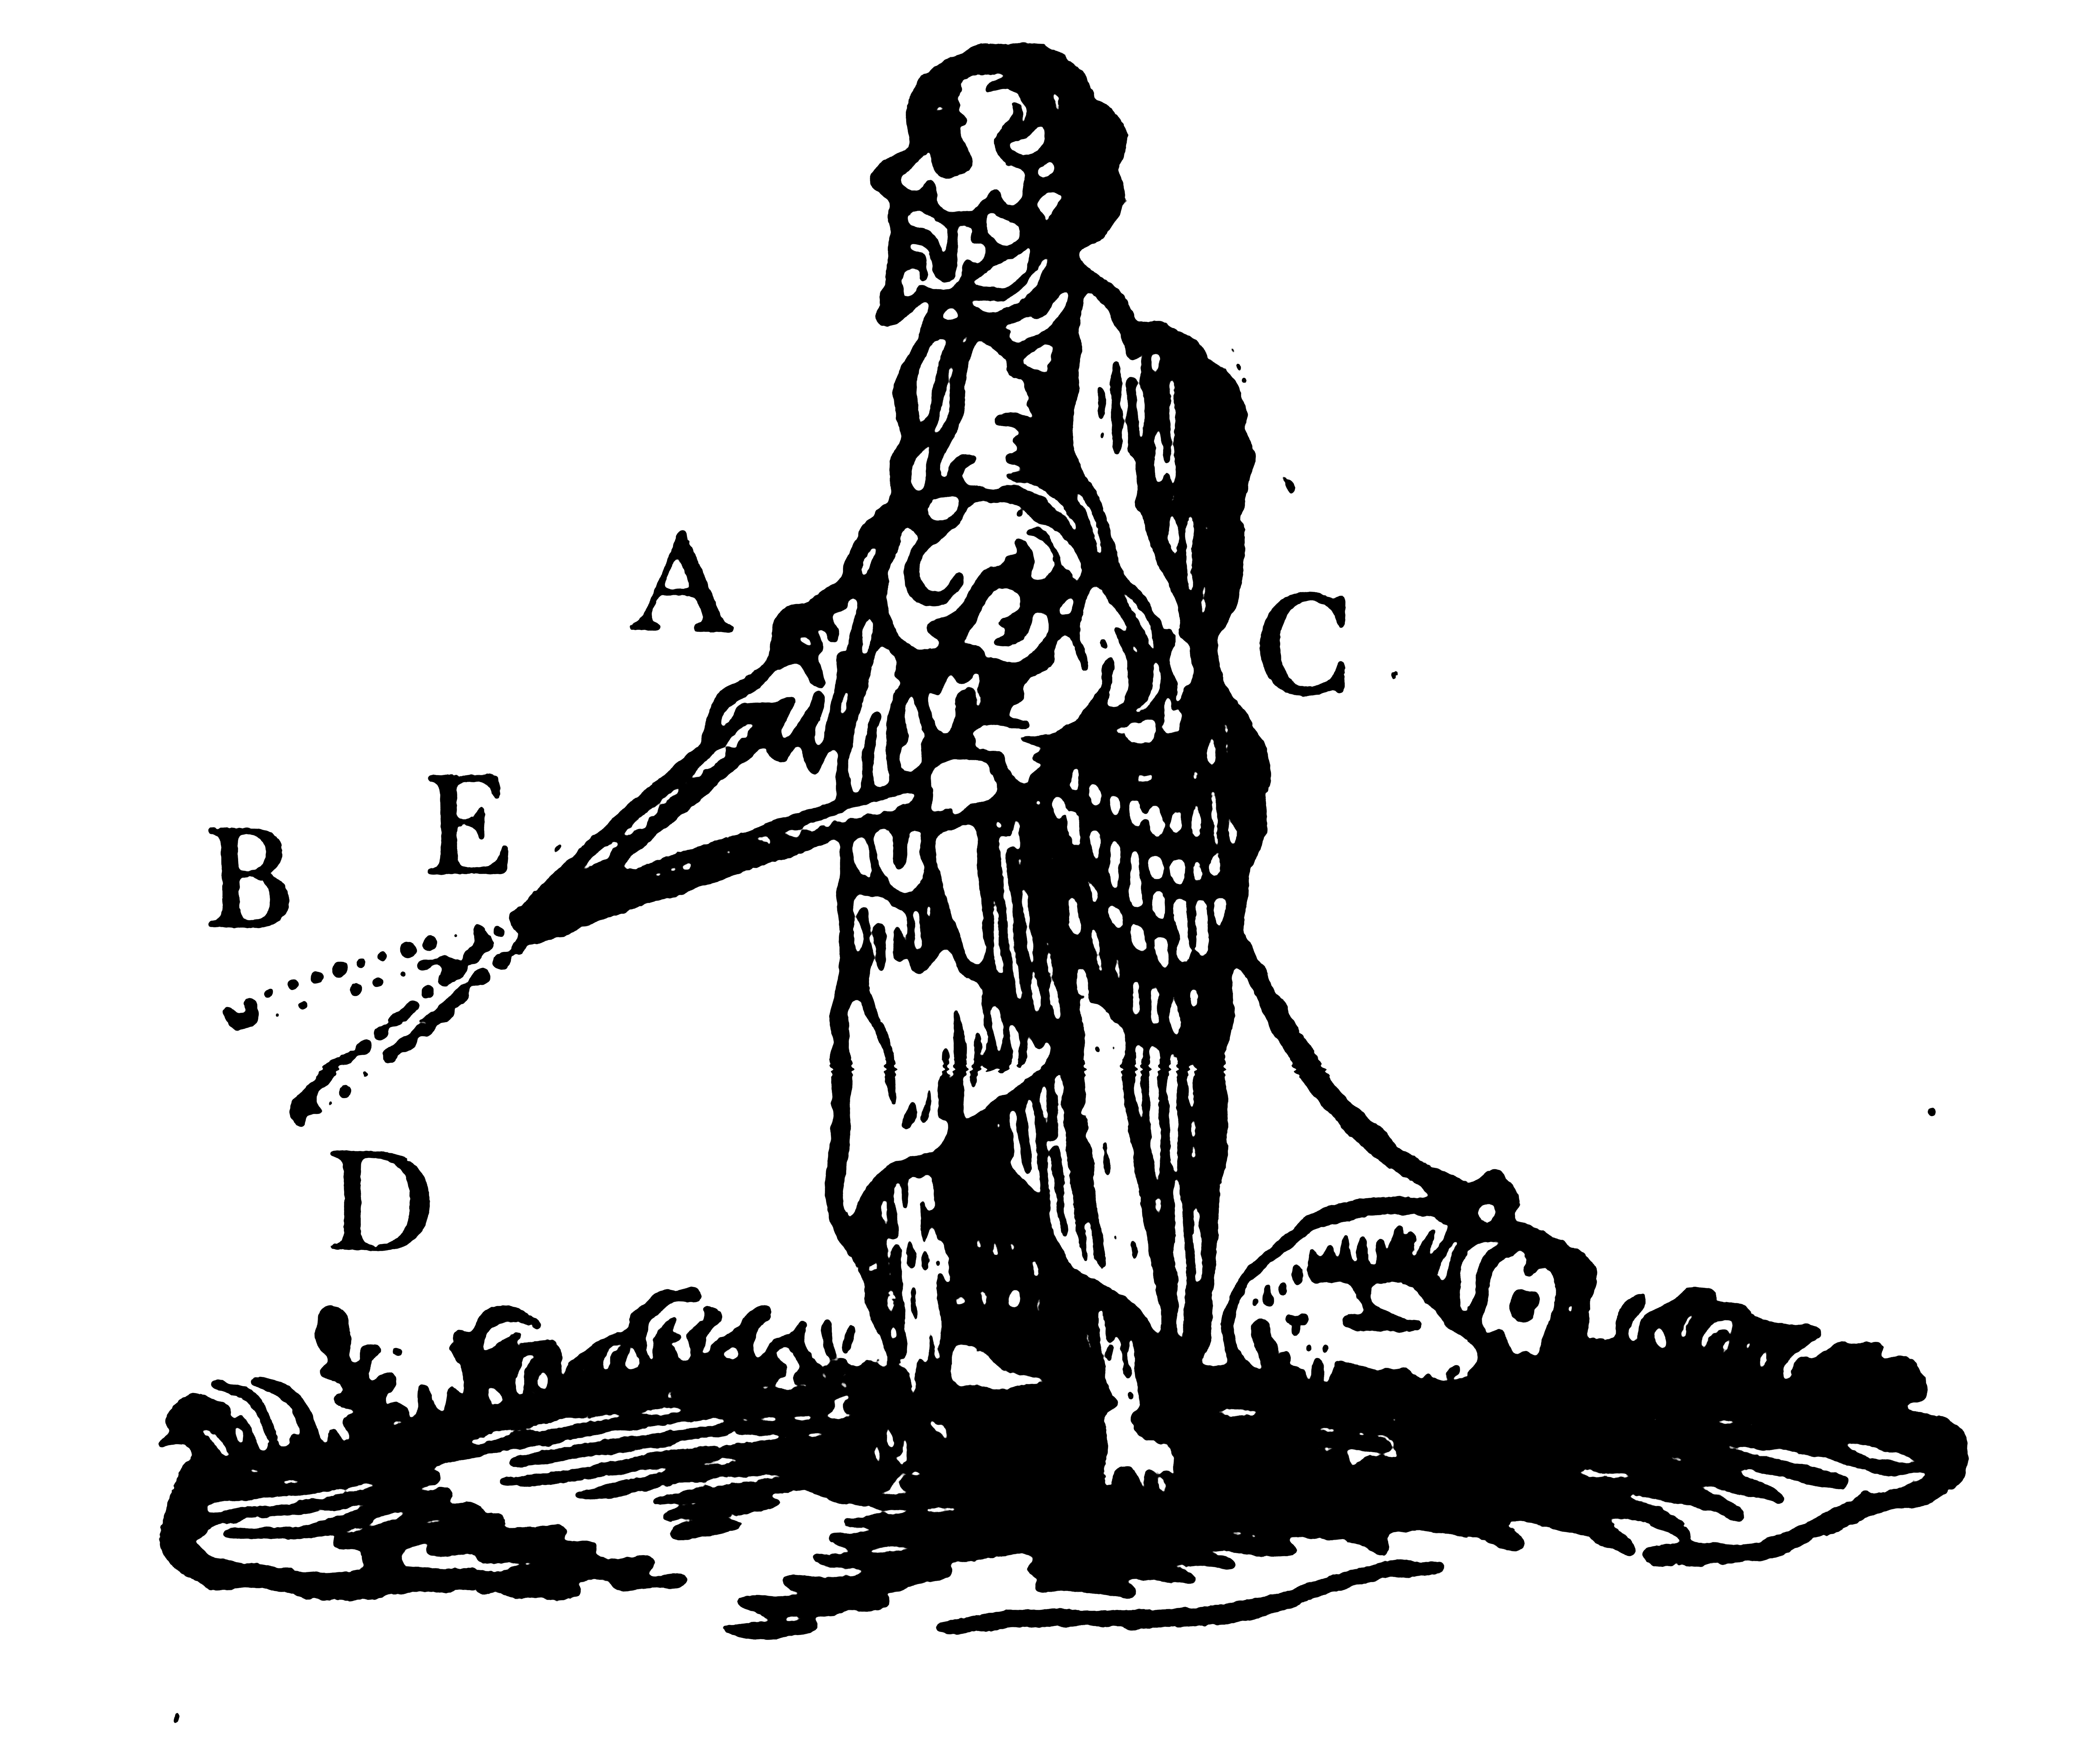
\includegraphics[scale=2]{graphics/blind.jpeg}
% 	\caption{\citealt{Descartes:1637uq}}
% 	\label{fig:blind}
% \end{figure}

This is not without ancient precedent. Consider Democritus\index{Democritus}, at least as presented by Sextus Empiricus\index{Sextus Empiricus} (\emph{Adversus Mathematicos}, \textsc{vii}). Linguistic conventions may license, in certain circumstances, our predicating ``white''\index{white} of the sun\index{sun} given the character of the sensory experience that it elicits, but there is nothing corresponding to this predication over and above our sensory reaction to atomic stimuli. What is novel in early modern thinking about sensory experience is not the idea that the causes of color perception do not resemble the colors that perception purports to present. That idea is present in the ancient atomists and arguably has Parmenidean\index{Parmenides} roots. What is novel about the early modern period is the enthusiasm with which this doctrine was met, and the widespread consensus that emerged, a consensus that remarkably persisted for four centuries. It is only against the background of such a consensus that \citet[]{Hume:1748zr}\index{Hume, David} can claim that it takes but the slightest bit of philosophy to show that there are no colors that inhere in bodies that resemble our impressions of them. While there may be ancient precedent for this doctrine, there is nothing like the modern consensus in the ancient world. There is no ancient correlate of the modern paradigm that would render intelligible Hume's dismissiveness. Aristotle himself is an important and notable dissenter. As the great defender of the manifest image in the classical world, Aristotle defends a pre-Parmenidean perceptual realism by post-Parmenidean means. (For a recent different account of these matters see \citealt{Lee:2011ys}.)\index{wax analogy}

Colors that constitutively shape\index{shaping!constitutive} visual experience may be causes of such experiences, but the character of our visual experience depends upon and derives from the character of the color\index{color} presented to our point of view\index{perspective}. In this sense does the perceptual experience come to resemble its object in assimilating its sensible form\index{assimilation!of sensible form}. Should color\index{color} experience not resemble, in the relevant sense, the colors that are their objects, then colors would shape our visual experience merely causally, as Democritus\index{Democritus} and Descartes\index{Descartes, Ren\'{e}} maintained. According to Aristotle's perceptual realism, colors are causes of color perceptions that resemble them, by perceptions being the presentation of the colors, a presentation that constitutively shapes\index{shaping!constitutive} our visual consciousness.\index{wax analogy}

We have been discussing Aristotle's two remarks about the material aspect of the wax analogy\index{wax analogy}: (1) that the wax\index{wax} takes on the impression\index{impression} of the signet ring\index{signet ring} without the bronze\index{bronze} or the gold\index{gold}, and (2) that the bronze or gold signet ring produces the impression\index{impression} but not qua bronze or gold. The first remark is the summation of Aristotle's case against the Empedoclean principle\index{Empedocles!the Empedoclean principle}. Color perception may be the assimilation of chromatic form, but nothing material is assimilated. The second remark is the expression of a color realism\index{color!realism} that was rejected by early modern thinkers---not only by Descartes\index{Descartes, Ren\'{e}}, but by a diverse group of thinkers that includes Galileo\index{Galileo Galilei}, Locke\index{Locke, John}, Boyle\index{Boyle, Robert}, and others as well. According to this premodern realism\index{realism}, it is the color\index{color} of the particular\index{particular} and not its matter that primarily explains the perception of its color. Colors are causes of color perceptions that resemble them, in the sense in which they can, by color perception being the presentation of color to the perceiver's point of view. Color's presence\index{presentation} in visual awareness shapes the experience that affords that awareness in that its character depends upon and derives from the character of the presented color. Nevertheless, consistent with this, color is the cause of its presentation in perception. Color, being the power\index{power} to affect light\index{light}, has the derived power to mediately affect the organ of sight by affecting the intervening medium. In altering the character of the illumination in the eye's\index{eye} interior, color triggers the reactive capacity\index{capacity!reactive} for sight whose exercise is the presentation\index{presentation} in visual awareness of that color. Like a wind\index{wind} causing a fire\index{fire} to burn in its direction, color\index{color} causes a perceiver to stand in a perceptual relation to it, that of visual awareness. And in being so presented in visual awareness color constitutively shapes color experience.
\index{assimilation!without matter|)}\index{wax analogy}

% subsection without_matter (end)

\subsection{Sensory Presentation as a Mean} % (fold)
\label{sub:sensory_presentation_as_a_mean}

After offering the definition of perception\index{perception!definition}, Aristotle writes:
\begin{quote}
	A primary sense-organ is that in which such a power is seated. The sense and its organ are the same in fact, but their essence is not the same. What perceives is, of course, a spatial magnitude\index{magnitude}, but we must not admit that either the having the power to perceive or the sense itself is a magnitude; what they are is a certain form or power in a magnitude. (Aristotle, \emph{De Anima} \textsc{ii} 12 424\( ^{a} \)24--28; Smith in \citealt[43]{Barnes:1984uq})
\end{quote}
A sensory capacity and its sense organ are the same. It is at least the case that no animal has that sensory capacity unless they also have the relevant sense organ. Nevertheless sensory capacities and their sense organs are essentially different. Sense organs have magnitudes whereas sensory capacities do not. Recall it was by reflecting on virtues and capacities that the Eleatic Visitor\index{Eleatic Visitor} elicits a refinement of the Giants'\index{Giants} metaphysics. The palpable remains real, but not only the palpable is real. The Giants are thus led to recognize the being of capacity\index{capacity}. Sense organs must have magnitudes\index{magnitude} if they are to be mediately acted upon by distal sense objects. A medium\index{medium} in contact with the sense organ is what acts upon it, and the sense organ must have spatial magnitude for this to be the case. But a sensory capacity, being a power\index{power} or potentiality\index{potential}, lacks spatial magnitude. Sensory capacities and sense organs may be united in the animal that possesses them, but they are essentially distinct. Sensory capacities are a certain form or power in magnitude. Sensory capacities are no warrior senses within the insensate Wooden Horse. It is the animal that sees and not their eyes. Nevertheless, the capacity to see is united with the organ of sight. It is only in that particular spatial magnitude, the eyes that naturally and harmoniously occur as a parts of the whole and healthy animal, that the animal's capacity to see resides.

% In the last line of the quoted passage, Smith translates \emph{logos} as form, the more usual Greek for form being \emph{eidos}. Importantly, at least in some contexts, \emph{logos} can also be understood as ratio. This latter reading of \emph{logos} can seem apt, when we consider the explanatory consequences of the claim that sensory capacities are a certain logos or power in a spatial magnitude, the organ of sensation:

That the animal's\index{animal} capacity to perceive is a certain form\index{form} or power\index{power} in a spatial magnitude\index{magnitude} echoes an important earlier claim. Aristotle explains what the soul\index{soul} of an animal\index{animal} is by means of an analogy with artifacts and parts of animals. If the eye\index{eye} were an animal, then the capacity to see would be both essential to it and its soul. Moreover this claim is understood in terms of Aristotle's hylomorphic theory: ``sight is the substance of the eye which corresponds to the account, the eye being merely the matter of seeing'' (\emph{De Anima} \textsc{ii}\index{De Anima@\emph{De Anima}}; Smith in \citealt[]{Barnes:1984uq}). Sight\index{sight} is the form\index{form} and substance\index{substance} of the eye\index{eye}, the material parts of the eye---the membrane\index{membrane}, the internal water\index{water!internal}---the matter\index{matter}. On the hylomorphic theory, matter is a kind of potentiality\index{matter!as potentiality} and form a kind of actuality\index{form!as actuality}. The matter\index{matter} of the eye\index{eye} is potentially an eye since it is capable of taking on the form of an eye, by sustaining a transparent passage\index{eye!passages leading within} to the perceptive part of the soul\index{soul!perceptive part within} so that it may be mediately acted upon by color\index{color} and so ground the reactive capacity\index{capacity!reactive} for sight\index{sight}. When interior water\index{water!internal} is bound by the membrane\index{membrane} and the other parts of the eye are suitably arranged, the matter in taking on the form\index{form} that it does, in so acquiring the capacity for sight, actualizes this potentiality. The animal's\index{animal} capacity to perceive is in a spatial magnitude\index{magnitude}, the sense organ with which it is united, in a specific technical sense. The capacity to perceive is the form\index{form} of the sense organ. It is only by the material parts of the sense organ taking on that form does it endow the animal with the relevant perceptual capacity. A perceptual capacity is united to its sense organ as form is to matter\index{matter}.

Given this interpretation, we can see how this passage is relevant to the definition of perception\index{perception!definition} that precedes it. Perception so defined was a power or potentiality, the perceiver's power\index{power} or potential\index{potential} to become like the perceived object is actually. In assimilating the sensible form\index{assimilation!of sensible form} of the object, the sense, being a form or power lacks magnitude\index{magnitude}. Thus the relevant assimilation could not be the enmattering of the sensible form\index{form} in the perceptive part of the soul of the perceiver. The sense being a form or power has no matter to in-form. Consider, again, the smith's\index{swordsmith} production of the sword\index{sword}. In producing the sword, the iron\index{iron} takes on the form\index{form} of the sword\index{sword} contained in the soul\index{soul} of the smith possessing the art\index{art} of sword-making. The form of the sword exists in the soul of the person possessing the art but not as enmattered. There is no sword in the smith's soul. And there is no color in the perceiver's soul. Yet each are \emph{relata} of correlative qualitative assimilations. The senses may assimilate sensible form but not by enmattering it.

According to Aristotle, that the capacity to perceive is a certain form\index{form} or power\index{power} in a spatial magnitude\index{magnitude}, understood as the organ of sensation, has two explanatory consequences:
\begin{quote}
	This enables us to explain why excesses in objects of sense destroy the organs of sense; if the movement set up by an object is too strong for the organ, the form which is its sensory power is disturbed; it is precisely as concord\index{concord} and tone\index{tone} are destroyed by too violently twanging the strings of a lyre\index{lyre}. This explains also why plants\index{plant} cannot perceive, in spite of their having a portion of soul\index{soul} in them and being affected by tangible objects themselves\index{the tangible}; for their temperature\index{temperature} can be lowered or raised. The explanation is that they have no mean\index{mean}, and so no principle in them capable of taking on the forms of sensible objects but are affected together with their matter. (Aristotle, \emph{De Anima} \textsc{ii} 12 424\( ^{a} \)28--424\( ^{b} \)3; Smith in \citealt[43]{Barnes:1984uq})
\end{quote}
The claim that a sensory capacity is a form\index{form} or power\index{power} in a spatial magnitude\index{magnitude}, understood as the organ of sensation naturally occurring as a part of the healthy animal\index{animal}, is a key part of two explanations. First, that claim is meant to explain why if the movement set up by an object is too strong for the organ, its sensory power is disturbed. And second, that claim is meant to explain why plants\index{plant} cannot perceive. Let us consider these in turn.

``If the movement set up by an object is too strong for the organ, the form which is its sensory power is disturbed.'' Why should this be so? Begin with the movement. The movement is set up by an object, presumably, the object of perception. It is not the object's movement, but a movement set up by the object, that is said to too strongly affect the sense organ. A movement set up by an object is the object of perception mediately acting upon the sense organ of a suitably placed, awake, attentive perceiver by acting upon an intervening medium. In the case of seeing\index{seeing} in light,\index{light} color\index{color} is the primary object of sight. What is too strong for the eye\index{eye} would be, not the color's movement, the manner in which it moves and acts upon the external transparent medium, by altering the character of its illumination, but the movement set up by the color, a movement conveyed by the external medium to the transparent medium\index{medium!internal} within the eye's interior, the external light\index{light} extended within. In the case of vision, the movement that is too strong for the eye is the color of a remote external particular mediately acted upon the transparent water within the eye's interior. Not only does light enables us to see the scene before us, but if it is particularly intense, it can blind us to the scene as well. Sorenson provides a nice example:
\begin{quote}
	The \emph{Krak Des Chevaliers}\index{Krak Des Chevaliers@\emph{Krak Des Chevaliers}} (Castle of Knights) in Syria has a covered passageway. When visitors travel through the long stretch of darkness, they emerge suddenly in daylight. The passageway was designed to dazzle invaders. \citep[6]{Sorensen:2008kx}
\end{quote}

It is the strength of the movement conveyed to the eye's\index{eye} interior that disturbs the sensory power\index{power} which is its form\index{form}. The strength of the movement affects the sense organ not the soul\index{soul}. One of the lessons from Book \textsc{i} was that the soul does not move. If the soul does not move, it cannot be acted upon. The organ of sensation, being a bodily magnitude\index{magnitude}, may, however, be acted upon. Moreover, in order for the sense organ to function, to endow the perceiver with the relevant sensory capacity it must naturally occur harmoniously\index{harmony} as a part of the healthy animal\index{animal}. We have an echo here of Empedocles'\index{Empedocles} cosmology. Recall at a certain stage of the cosmic cycle animal parts appear, though in a disordered state. These combine giving rise to fantastical animals that could not reproduce and tended not to survive. However, due to an increase in Aphrodite's\index{Aphrodite} Love\index{Empedocles!Love}, when the parts of the animals are harmoniously combined, this fits them to life in their natural environment and they gain the ability to reproduce. It is Aphrodite's Love, the principle of harmony\index{harmony}, obtaining among the parts of animals\index{animal} that enables them to properly function thus fitting the animal to life in its environment. Despite rejecting the harmony conception of the soul in Book \textsc{i}, Aristotle retains this aspect of Empedocles'\index{Empedocles} cosmology. In part it is the organ's relation to the perceiver that allows it to endow the perceiver with the relevant sensory capacity. The strength of the movement conveyed to the eye's interior acts upon the eye\index{eye} so as to change this relation. Overly intense illumination taken within the eye's interior loosens the form of the eye, the capacity to see by means of it, thus blinding the perceiver. Throughout this process, the perceptive part of the soul remains unaffected, remaining ready to assimilate sensible form as soon as the eye returns to a functioning state.

It is extreme sensible objects, too loud\index{loud} a noise, too bright\index{bright} a light\index{light}, whose mediate action upon the internal medium\index{medium!internal} disturbs the functioning of the relevant sense organ, in fortunate circumstances, only temporarily. Notice also it is the positive extreme of the range of qualities that disorders the sense organ's functioning. It is too loud a sound\index{sound} and not too still a silence\index{silence} that deafens. It is too bright a light and not too dark\index{dark} a night that blinds. It is the extreme positive determinants of sensible qualities\index{sensible qualities} and not their privation\index{privation} that loosens the form and power of the sense organ. This is why Aristotle emphasizes the strength of the movement set up by the object. Aristotle explains this by means of analogy: ``it is precisely as concord\index{concord} and tone\index{tone} are destroyed by too violently twanging the strings of a lyre\index{lyre}.'' Just as it is the organ that is violently acted upon, it is the instrument that is violently acted upon. Moreover, just as the strength of the movement disrupts the functioning of the sense organ, the strength of the movement disrupts the functioning of the instrument, concord and tone are destroyed by too violently playing the lyre. Aristotle is describing a loss of attunement. Thus Hamlyn\index{Hamlyn, D.W.} argues:
\begin{quote}
	I do not think that, when Aristotle speaks of the consonance\index{consonance} of the strings of an instrument being destroyed by too violent a blow, the reference to consonance implies anything to do with the harmony\index{harmony} of different strings. It is the consonance and pitch of a single string which is destroyed when it is struck too violently; the string does not then sound properly at the right pitch and with the proper timbre\index{timbre}. \citep[114]{Hamlyn:2002ys}
\end{quote}
The lyre\index{lyre} in being played too violently loses its attunement\index{attunement}. Its string is loosened, and the lyre no longer functions as it should, the consonance\index{consonance} and pitch\index{pitch} of the string destroyed. Due to the operation of Strife, the parts of the instrument are no longer harmoniously\index{harmony} arranged making it no longer fit to be played. Similarly, the eye\index{eye} in being illuminated too violently loses its attunement. Its form is loosened, and the eye no longer functions as it should, its capacity to take in the environment destroyed. Due to the operation of Strife\index{Empedocles!Strife}, the eye is no longer harmoniously related to the animal\index{animal} in which it naturally occurs as a part making it no longer fit assimilate external color. 

Aristotle moves from the effects of extreme sensible objects on certain bodies\index{body}, sense organs, the spatial magnitudes\index{magnitude} in which sensory capacities reside, to the effects of sensible objects on bodies that are not themselves sense organs. That sense is a certain form or power in a spatial magnitude can explain why bodies that are not sense organs, that lack that form and power, do not perceive. Plants\index{plant}, unlike animate natural bodies\index{animal} with sense organs naturally and harmoniously\index{harmony} occurring as parts, do not perceive. Heat is a sensible object. And plants, while they may be heated, do not perceive heat. ``The explanation is that they have no mean\index{mean}, and so no principle in them capable of taking on the forms of sensible objects but are affected together with their matter'' (\emph{De Anima} \textsc{ii} 12 424\( ^{b} \)1--3; Smith in \citealt[43]{Barnes:1984uq}). 

Talk of ``mean''\index{mean}, here, is a back reference to the previous chapter, where the power to discriminate among tangible objects\index{the tangible} was explained as the power\index{power} to detect differences by a sort of mean\index{mean}:
\begin{quote}
	That is why we do not perceive what is equally hot\index{hot} and cold\index{cold} or hard\index{hard} and soft\index{soft}, but only excesses, the sense itself being a sort of mean\index{mean} between the opposites\index{opposites} that characterize the objects of perception\index{perception!object of}. It is to this that it owes its power of discerning the objects in that field. What is in the middle is fitted to discern; relatively to either extreme it can put itself in the place of the other. As what is to perceive white\index{white} and black\index{black} must, to begin with, be actually neither but potentially either (and so with all the other sense-organs), so the organ of touch\index{touch} must be neither hot\index{hot} nor cold\index{cold}. (Aristotle, \emph{De Anima} \textsc{ii} 11 424\( ^{a} \)1--10; Smith in \citealt[42]{Barnes:1984uq})
\end{quote}
An animal\index{animal} feels the warmth of a body\index{body} that it touches, in part, because the animal's flesh\index{flesh} is cooler\index{cold} than that body. The animal feels the warmth\index{hot} by noticing the difference in temperature\index{temperature} between it and the body that it feels. An argument from blindspots\index{blindspots} is offered on behalf of this: If the body that the perceiver's flesh\index{flesh} is in contact with is the same temperature, then the perceiver will not feel its temperature. Plants\index{plant} are natural beings. They have nutritive and reproductive capacities and thus are also animate, but they are insensate lacking the perceptive part of the soul\index{soul!perceptive part within}. The air\index{air} that surrounds them, or the earth\index{earth} in which they are implanted, may heat\index{hot} or cool\index{cold} them. But despite being animate natural beings\index{living beings} acted upon by sensible objects, plants\index{plant} do not perceive differences in temperature\index{temperature} and so do not feel hot\index{hot} or cold\index{cold}. What they lack, according to Aristotle, is a sort of mean\index{mean}. Animals\index{animal} may change in temperature\index{temperature}, but they have the ability to regulate their temperature. This more or less fixed regular temperature serves as the mean by which departures from it may be felt. But plants lack such a fixed regular temperature and so lack a mean by which differences in temperature may be perceived.

Is the notion of a mean\index{mean} at work in Aristotle's explanation of our ability to discriminate temperature\index{temperature} also meant to characterize sensory presentation more generally? Is it that plants\index{plant} lack a mean and thus a principle to assimilate temperature? Or is it that every principle for the assimilation of sensible form\index{assimilation!of sensible form} without matter\index{assimilation!without matter} essentially involves a mean\index{mean}? This issue is raised by the proximity of the back reference to Aristotle's general definition of perception. The argument from blindspots\index{blindspots} is only offered in the case of touch\index{touch}. Moreover, it works best with the tangible\index{the tangible} quality of temperature\index{temperature}. Is it really true, say, that it takes a hard\index{hard} hand to appreciate delicate softness\index{soft}? Moreover, the analogy with vision presented in the passage does not ascribe a mean at work in vision, rather something weaker is attributed---if the eye is to see white and black it must be neither. This is true. But the transparent\index{transparency} water\index{water!internal} in the eye's\index{eye} interior is neither some intermediate shade determined by an equitable ratio\index{ratio} of light\index{light} and dark\index{dark}. It does not have within itself the source of its own color\index{color} but is rather transparent\index{transparency}. Lacking a mean\index{mean} may make you insensible to differences in ambient temperature\index{temperature}, but this does not entail that all sensory capacities operate by discriminating from a mean. The plant\index{plant} being heated without being warmed is meant to have a different lesson.

The plant\index{plant} in being heated is acted upon and altered. An animal\index{animal} in feeling warmth\index{hot} is acted upon, but it undergoes only an alteration of a sort\index{alteration!of a sort}. Aristotle is thus emphasizing the central denial of \emph{De Anima} \textsc{ii} 5\index{De Anima@\emph{De Anima}}, that the exercise of our perceptual capacities is not a qualitative alteration\index{alteration}. In so doing he is also emphasizing a feature of the qualitative assimilation\index{assimilation!qualitative} at work in perception\index{perception}. The ambient air acts upon the plant\index{plant} and heats it, say. In being heated, the plant is altered. One quality of the plant has been destroyed and replaced by a contrary from the same range. In being altered in this way, the sensible form of heat is enmattered in the plant. Some commentators suggest that the plant is heated by taking in hot\index{hot} material\index{matter}, other suggest that heating requires no material assimilation\index{assimilation!material}. On either model, the sensible form of heat is enmattered in the plant\index{plant}. But the assimilation of sensible form\index{assimilation!of sensible form} in sense perception\index{perception} does not involve that form becoming enmattered in the perceptive part of the soul\index{soul!perceptive part within}, anymore than an enmattered sword\index{sword} resides in the soul\index{soul} of a person possessing the art\index{art} of making swords. Insensate plants\index{plant} are emphasizing that the constitutive shaping\index{shaping!constitutive} of sensory consciousness by its object does not require the sensible form be enmattered in the perceiver. So in perception\index{perception}, the perceiver, or perhaps their perceptual experience, assimilates the form without the matter of the remote external particular. The assimilation of sensible form\index{assimilation!of sensible form} occurs without matter\index{assimilation!without matter} in two ways. Perception involves a non-material mode of assimilation in that nothing material is taken in. To be palpable is to be imperceptible\index{to be palpable is to be imperceptible}. Assimilation may not involve taking in anything material but could still involve the assimilated sensible form in-forming the perceiver's matter. However, assimilation is non-material in this sense as well. Perception involves a non-material mode of assimilation in that the assimilated sensible form is not enmattered in the perceiver.

% subsection sensory_presentation_as_a_mean (end)

% section the_wax_analogy (end)

\section{The Resolution of Empedoclean Puzzlement} % (fold)
\label{sec:the_resolution_of_empedoclean_puzzlement}

Empedoclean puzzlement\index{Empedoclean puzzlement} about the sensory presentation\index{presentation} of the colors\index{color} of distal particulars\index{perception!at a distance} was due, in part, to Empedocles'\index{Empedocles} adherence to a general conception of sensory awareness for which ingestion provides the model\index{ingestion model}. Central to that model was the Empedoclean principle, to be perceptible is to be palpable to sense. Empedoclean puzzlement\index{Empedoclean puzzlement} about the sensory presentation\index{presentation} of color\index{color} consists in the apparent tension between two claims:
\begin{enumerate}[(1)]
    \item the objects of color perception are qualities of external particulars located at a distance from the perceiver; and\index{perception!at a distance}
    \item \emph{the Empedoclean principle}: to be perceptible is to be palpable to sense---in order for something to be the object of perception it must be in contact with the relevant sense organ.\index{Empedocles!the Empedoclean principle}
\end{enumerate}
Effluences\index{Empedocles!effluence} in Empedocles' theory of vision\index{Empedocles!perception} are meant to resolve this puzzle by explaining how the colors of remote external particulars may be palpable to the organ of sight. Distant objects may be sensed by sensing the material effluences they emit. If the color of an object is the material effluence that it emits\index{Empedocles!effluence!chromatic}, then the color\index{color} of a remote object can be assimilated and so be palpable to sight\index{ingestion}. Not only does Aristotle reject the theory of effluences, and with it Empedocles' own resolution of the puzzle, but he also rejects the principle that generated the puzzle that effluences were meant to resolve. Specifically, he rejects the Empedoclean principle\index{Empedocles!the Empedoclean principle}, to be perceptible is to be palpable to sense\index{to be perceptible is to be palpable to sense}. Far from being a material precondition for the sensing of color, contact precludes sensation. A colored particular's\index{particular} contact with the eye\index{eye}, the organ of sight, blinds the perceiver to that particular and its color. To be palpable is to be imperceptible. Aristotle's rejection of the Empedoclean principle\index{Empedocles!the Empedoclean principle} is a resolution of Empedoclean puzzlement\index{Empedoclean puzzlement}, at least in its original form, precisely by that puzzlement being generated by the tension between the that principle and the claim that the objects of color perception are qualities of external particulars located at a distance from the perceiver.

Aristotle, nevertheless, retains a conception of perception as a mode of assimilation even as he rejects the ingestion model\index{ingestion model}. The naturalness of thinking of seeing as taking in the external scene before one persists even after rejecting the Empedoclean principle\index{Empedocles!the Empedoclean principle}. This natural thought gives rise to a residual puzzlement. How can one take in what remains external? And if one can, what could taking in mean, here, such that one could? Empedoclean puzzlement, in its most general form, consists in the persistence of this latter question.\index{Empedoclean puzzlement!general form}

How can one take in what remains external? If the generalized form of the Empedoclean puzzlement consists in the persistence of this question\index{Empedoclean puzzlement!general form}, then Aristotle's definition of perception\index{perception!definition} can be understood to address this puzzlement precisely by offering an answer\index{Empedoclean puzzlement!general form}. A perceiver takes in what remains external by assimilating the chromatic form of the remote external particular while leaving its matter in place.\index{assimilation!of sensible form} Aristotle's definition of perception as the assimilation of sensible form without matter is meant to address the generalized form of Empedoclean puzzlement. It is meant to be the sense in which the perceiver takes in the scene before one. More specifically, it is meant to be the sense in which the perceiver takes in what remains external. 

In seeing, we take in the scene before us by assimilating the chromatic form of the particulars arrayed in that scene, by our experience being constitutively shaped\index{shaping!constitutive} by their color. In chapter~\ref{sec:the_general_characterization_of_perception}, the epistemological significance of this doctrine was stressed.\index{perception!objectivity} If the perceiver becomes like the way the perceived object actually is, in the sense that their perceptual experience is constitutively shaped by that object, then it is impossible for their experience to be as it is and that object be some way other than it actually is at least in sensible respects. The assimilation of sensible form thus underwrites the objectivity of perceptual content. Moreover, this objectivity is achieved quite independently of any spatial contact with the object of perception. In Aristotle's definition, the qualification, without matter, emphasizes just this point. Only matter is spatially located, and thus only matter may be in contact with the organ of sensation.\index{assimilation!without matter}

The perceiver assimilates the chromatic form of the perceived particular and so becomes like that particular actually is prior to perception. The perceiver, or perhaps their perceptual experience, becomes like the colored particular in that their visual experience is constitutively shaped\index{shaping!constitutive} by the presentation\index{presentation} of that color\index{color} to their point of view\index{perspective}. In being constitutively shaped by the color of the perceived particular\index{particular}, the visual experience of the perceiver may become like the particular actually is in chromatic respects, but this does not mean that they or their perceptual experience is exactly like the perceived object. So being constitutively shaped by the presented color does not require that in seeing the sun the perceiver becomes actually white.

The likeness involved in the visual assimilation\index{assimilation!qualitative} of color\index{color} concerns the qualitative character of visual experience and the way that it depends upon and derives from the qualitative character of the object of that experience, the color presented to the perceiver's point of view\index{perspective}. Qualities\index{quality}, like the brilliant white\index{white} of the sun\index{sun}, like states\index{state}, lack locations\index{location}. Colors may only inhere in located things with extensive magnitudes\index{magnitude}, but the colors are at best indirectly located where they inhere. Colors, being qualities, lack location and so are not at a distance from the perceiver, at least not directly.\index{state!precludes space-occupancy} There is neither the need for, nor the possibility of, the color of a remote particular traveling the spatial gap between that particulars and the perceiver. Qualitative assimilation\index{assimilation!qualitative} lacks the spatial presuppositions that makes the material assimilation of remote objects seem problematic.

Understanding assimilation, not as it figures in the ingestion model\index{the ingestion model}, as a mode of material assimilation\index{assimilation!material}, but on the model of qualitative alteration\index{alteration}, thus bears on Empedoclean puzzlement\index{Empedoclean puzzlement} in two ways. First, it bears on the original form of the puzzlement in that qualitative assimilation lacks the spatial presuppositions that makes the material assimilation of remote objects problematic. That is merely a negative claim about sensory presentation, that it lacks a feature that made the sensory presentation of remote objects seem problematic. But importantly, Aristotle, in his definition, is also making a positive claim.\index{Empedoclean puzzlement!general form} In seeing the brilliant white\index{white} of the sun\index{sun}, the perceiver may take in the color of the sun consistent with its being distant. The sun remains in the heavens\index{heaven} even as it shapes\index{shaping!constitutive} the perceiver's experience of it. Talk of taking in may be a phenomenologically apt\index{phenomenology} description of the perceiver's experience of the color of the sun\index{sun}, but what does taking in mean, here, if it is not a material mode of assimilation? Aristotle positive claim provides an answer, and one that is consistent with the object of visual experience remaining remote. 

Taking in the scene before one is not a mode of material assimilation\index{assimilation!material}, it is a mode of qualitative assimilation\index{assimilation!qualitative} akin to, but distinct from, the qualitative assimilation involved in qualitative alteration\index{alteration} (chapter~\ref{cha:two_kinds_of_potentiality}). Perception\index{perception} is like qualitative alteration\index{alteration} in that the perceiver must be acted upon to exercise their perceptual capacities and that this exercise involves a mode of qualitative assimilation, but crucial differences remain. The exercise of our perceptual capacities may involve qualitative assimilation\index{assimilation!qualitative}, but it is not the destruction of something by its contrary\index{destruction of something by its contrary}, the replacement of one quality\index{quality} by a contrary\index{contraries} from a common genus\index{genus}, but a preservative change\index{preservative change}. This is a kind of perfection\index{perfection}---in exercising their perceptual capacities, the perceiver realizes their nature as a perceiver. And whereas the motion of qualitative alteration\index{alteration} is incomplete\index{incomplete}, the relevant potentiality\index{potential} exhausted in its realization, perceptual activity\index{actual} is complete\index{complete} at every instance, its potentiality preserved. In seeing the brilliant white\index{white} of the sun, the perceiver both sees and has seen. Moreover, qualitative assimilation\index{assimilation!qualitative} in the case of vision does not require the perceiver to become exactly like the way the perceived object is prior to perception. The visual experience of the perceiver may be constitutively shaped\index{shaping!constitutive} by the color\index{color} of the sun\index{sun} and so like it, in some relevant sense, but not by the perceiver becoming white within. Moreover, qualitative assimilation\index{assimilation!qualitative} in the case of vision, if not in the case of alteration\index{alteration}, is relative to a point of view\index{perspective}\index{perception!viewpoint conception}. The perceiver takes in the white\index{white} of the sun\index{sun} by the perceiver, or perhaps their perceptual experience, becoming like the way the sun is actually like, brilliant white---by the sun's brilliant whiteness constitutively shaping their visual consciousness in being presented to their point of view.

It is these further positive claims that constitute Aristotle's resolution of the generalized form of Empedoclean puzzlement\index{Empedoclean puzzlement!general form}. Even if we grant that we can take in what remains external, we can still be puzzled about what talk of taking in, here, means such that we could. Aristotle's definition of perception\index{definition} is a resolution of this residual puzzlement precisely by offering an answer: In seeing we take in the color of the remote external particular by our experience becoming like the color presented to our point of view, by that color, presented in that way, constitutively shaping our visual consciousness.

Not only does Aristotle's positive claim provide an answer to what taking in amounts to when we take in the external scene by seeing it, but it also provides the basis of explaining the enduring appeal of talk of taking in or assimilation.\index{assimilation}\index{perception!objectivity} In seeing the brilliant white\index{white} of the sun\index{sun}, we take in the color\index{color} of that heavenly body by our experience becoming like the sun actually is, by its color constitutively shaping our visual consciousness in being presented to our point of view. In perceiving we become like the perceived object actually is. The objectivity of perception\index{perception!objectivity} consists in its being a mode of assimilation. If there is nothing that visual experience becomes like, if there is nothing it assimilates to, then it would not be a mode of assimilation and, hence, not a mode of perception. The perceiver's perceptual experience could not be as it is if a Cartesian demon\index{Cartesian demon} eliminated the perceived object. If perception is a mode of assimilation, then the visual experience that the perceiver undergoes in seeing a particular could not be as it is if that particular differed in visible respects relative to the perceiver's point of view.

What was compelling, all along, about the rhetoric of assimilation\index{assimilation} was its pretension to objectivity\index{perception!objectivity}. The Giants\index{Giants} were rightly impressed by the reality of what can be handled and offers resistance to touch\index{touch} (Plato\index{Plato}, \emph{Sophist} 246\( ^{a} \)\index{Sophist@\emph{Sophist}}; see chapters~\ref{sec:empedoclean_puzzlement} and \ref{sub:particular}). In understanding taking in as a mode of qualitative assimilation\index{assimilation!qualitative} akin to, but distinct from, the qualitative assimilation involved in qualitative alteration\index{alteration}, Aristotle provides proof of the pretended objectivity. If the perceiver becomes like the way the perceived object actually is, in the sense that their perceptual experience is constitutively shaped by that object as presented to their point of view, then it is impossible for their experience to be as it is and that object be some way other than it actually is at least in sensible respects.

Consider grasping\index{grasp} a solid body\index{body}. In handling that body it offers resistance to touch\index{touch}. Being solid\index{solid}, it retains its shape\index{shape}, a shape that the grasping hand conforms to. The Giants'\index{Giants} grasping\index{grasp} of rocks\index{rocks} and trees\index{trees} is a powerful rhetorical gesture. Grasping something which offers resistance to touch is a phenomenologically vivid and primitively compelling experience of what is external to us. If Boswell\index{Boswell, James} is to be believed, Dr Johnson's\index{Johnson, Samuel} performance outside of a church in Harwich\index{Harwich} belongs to the rhetorical tradition inaugurated by the Giants\index{Giants}: 
\begin{quote}
	After we came out of the church, we stood talking for some time together of Bishop Berkeley's\index{Berkeley, George} ingenious sophistry to prove the non-exist\-ence of matter, and that every thing in the universe is merely ideal. I observed, that though we are satisfied his doctrine is not true, it is impossible to refute it. I never shall forget the alacrity with which Johnson answered, striking his foot with mighty force against a large stone, \'till he rebounded from it, ``I refute it \emph{thus}.'' This was a stout exemplification of the \emph{first truths} of \emph{Pere Buffier}\index{Buffier, Pere}, or the \emph{original principles} of Reid\index{Reid, Thomas} and Beattie; without admitting which, we can no more argue in metaphysicks, than we can argue in mathematicks without axioms. To me it is inconceivable how Berkeley can be answered by pure reasoning \ldots\ \citep[\textsc{i} 471]{Boswell:1935fk}
\end{quote}
The reality of external matter was demonstrated in the resistance it offered to Dr Johnson's\index{Johnson, Samuel} foot, which rebounded despite its mighty force. It was a demonstration not in the sense of proof, since it is inconceivable how Berkeley\index{Berkeley, George} can be answered in pure reasoning. Moreover, what was stoutly exemplified was metaphysically axiomatic, a first truth, but proof proceeds from axioms, it does not establish them. Rather Dr Johnson's\index{Johnson, Samuel} performance was a demonstration of first truths by showing or exhibiting them (on the character of Johnson's refutation of Berkeley see \citealt{Patey:1986uq}). The incident reported by Boswell\index{Boswell, James} thus dramatizes an important part of the Giants'\index{Giants} doctrine---that the palpable is real---even if it fails to dramatize the whole of that doctrine---that only the palpable is real.
 
Grasping\index{grasp} is an important trope in the rhetoric of objectivity\index{perception!objectivity}. But notice that even the Giants'\index{Giants} grasping of rocks\index{rocks} and trees\index{trees} involved a mode of assimilation\index{assimilation}. Consider the way their hands assimilated to the shape of the rocks\index{rocks} and trees\index{trees} they grasped\index{grasp}. It is precisely our perceptual experience assimilating to its object that is the source of its objectivity\index{perception!objectivity}.  Grasping may be a paradigm case of sensory presentation\index{presentation}, but not because it involves an object being in contact with a sense organ. Rather, it is a paradigm case because the grasping\index{grasp} hand assimilates to the object grasped, and thus the objects grasped are presented to us as being independent of our grasping them. But suitably understood, this is a feature of all perceptual experience:
\begin{quote}
	For sensation is surely not the sensation of itself, but there is something beyond the sensation, which must be prior to the sensation (\emph{Metaphysica} \( \Gamma \) 6 1011\( ^{a} \)1; Ross in \citealt[56]{Barnes:1984kx}).\index{Metaphysica@\emph{Metaphysica}}
\end{quote}
For a sensory experience to be perceptual is for it to assimilate the sensible form actually instantiated by its object. This is what underwrites the objectivity of perceptual content.\index{perception!objectivity} Tactile descriptions of non-tactile modes of sensory awareness are thus emphasizing the objective presentation of their objects.

Aristotle's explanation of the objectivity of perception\index{perception!objectivity}, and his premodern perceptual realism\index{realism}\index{color!realism} more generally, is lost by the early modern period. Insofar as the early moderns deny that our sensory ideas resemble the objects that elicit them, they deny, as well, that sensory experience is a mode of qualitative assimilation. Insofar as sensory experience is no longer understood as the assimilation of the sensible form actually instantiated by an external particular, the moderns no longer have available to them the Aristotelian explanation of perceptual objectivity. As the modern paradigm reaches the stage of normal science, perceptual presentation\index{presentation} is replaced by the \emph{simulacrum} of ``sheer receptivity\index{receptivity}'' \citep[16]{Sellars:1967uq}\index{Sellars, Wilfrid}. The reliable differential responsiveness of sensation usurps the role previously played by sensory presentation. (For contemporary discussion of these matters see \citealt{McDowell:1998vn} and \citealt{Kalderon:2011fk}; for its history see \citealt{Hamlyn:1961ys}.)

According to a form of skepticism found within the phenomenological tradition, modern philosophy is ultimately unsustainable because of its adherence to the metaphysics of presence\index{metaphysics of presence}. If the metaphysics of presence cannot be coherently sustained within modern philosophy, at least with respect to sensory presentation\index{presentation}, this is not because of any contradiction or incoherence within the metaphysics of presence, but because modern philosophy abandoned sensory presentation from the beginning. If perception does not resemble its object, then perceived object does not constitutively shape\index{shaping!constitutive} the perceiver's experience, and so that experience could not consist in that object's sensory presentation. Moreover, the idea that colors\index{color} are, in some suitable sense, secondary qualities\index{secondary qualities} depends upon the perceiver's visual experience not resembling its external cause. The modern conception of colors as secondary qualities only arises in a philosophical context where Aristotle's premodern realism\index{realism}\index{color!realism} has been abandoned and, with it, sensory presentation itself. Colors only seem secondary when color experience is conceived as a mode of sheer receptivity\index{receptivity} rather than a mode of sensory presentation\index{presentation}.

Consider the revulsion Melville\index{Melville, Herman} expresses for Locke's \citeyearpar{Locke:1706hc}\index{Locke, John} metaphysics. In an extended meditation on the whiteness\index{white} of the Whale\index{Whale} as the source of mortal terror\index{mortal terror}, Mellville consider's Locke's view that colors are secondary qualities having just discussed Newton's\index{Newton, Issac} theory of color\index{color}:
\begin{quote}
	And when we consider that other theory of the natural philosophers, that all other earthly hues\index{hue}---every stately or lovely emblazoning---the sweet tinges of sunset skies and woods; yea, and the gilded velvets of butterflies, and the butterfly cheeks of young girls\index{butterfly cheeks of young girls}; all these are but subtile deceits, not actually inherent in substances\index{substance}, but only laid on from without; so that all deified Nature absolutely paints like the harlot\index{harlot}, whose allurements cover nothing but the charnel-house\index{charnel-house} within \ldots\ \citep[ch. 42]{Melville:1851ms}
\end{quote}
Experience presents itself as the presentation\index{presentation} of particulars\index{particular} whose natures and powers\index{power} are independent of their being perceived. But if it does, then it is misleading in this regard. The apparent colors of things are but subtile deceits laid on from without\index{color!subtile deceits laid on from without} for nothing in our phenomenologically vivid color experience resembles its external cause. It is the absence of colors inherent in substances\index{substance} that Melville expresses revulsion for (like \citealt[chapter one]{Bergson:1912pi}\index{Bergson, Henri}, it is the modern conception of matter that Melville finds incredible.). And he represents this color nihilism as a fall from innocence. (For a different interpretation of the Lapsarian myth\index{Lapsarian myth} as applied to these matters, one given from within the modern paradigm, see \citealt{Chalmers:2006kx}.) We move from the butterfly cheeks of young girls\index{butterfly cheeks of young girls} to the painted harlot\index{harlot} whose allurements cover nothing but the charnel-house\index{charnel-house} within. I suspect that the ``charnel-house'' is less an expression of misogyny or New England prudery, but Melville\index{Melville, Herman} further echoing the Lapsarian myth\index{Lapsarian myth}. Death comes East of Eden. The Fall\index{The Fall|see also{Lapsarian myth}} changes our relationship with mortality, and with it, our relationship with ourselves. This absence\index{absence}, and the morbidity of its description, is emotional resonant in the context of the chapter, echoing, the way it does, God's absence. It is because the whiteness\index{white} of the Whale\index{Whale} signifies the absence of God\index{God} that it inspires mortal terror\index{mortal terror} in those who behold it. Experiencing God's absence is also a kind of fall\index{Lapsarian myth}, and one that changes our relationship with mortality. And it is precisely this that was the source of terror. But if color is absent in the external world, the way the whiteness of the Whale intimates that God may be, then our visual experience could not be as it presents itself as being, as the presentation\index{presentation} of the colors that inhere in remote external particulars.

% section presence_and_modernity (end)

% chapter form_without_matter (end)
